\documentclass{article}
\usepackage[utf8]{inputenc}

\title{Advanced Programming Labwork 8}
\author{Tom HERBRETEAU }
\date{November 2018}

\usepackage{natbib}
\usepackage{graphicx}
\usepackage{pgfplots}
\pgfplotsset{compat=newest}

\begin{document}

\maketitle
Every performance measures are done on ICT4 with eiffel.jpg, without counting the image saving.
\section{Introduction}
We have to convert the input image in HSV format, and then reconvert it in RGB format.
\section{Implementation}
There is two kernels, for each conversion.
I use a struct containts 3 arrays of double. To allocate the device memory for the struct, we need 3 cudamalloc, for each pointer in the struct. The struct will contain the converted input in HSV format. The conversion could be optimize by using mathematics ways to avoid BAD UGLY IF.

\section{Result}
The program last around 37ms to process the two conversions.
\newline
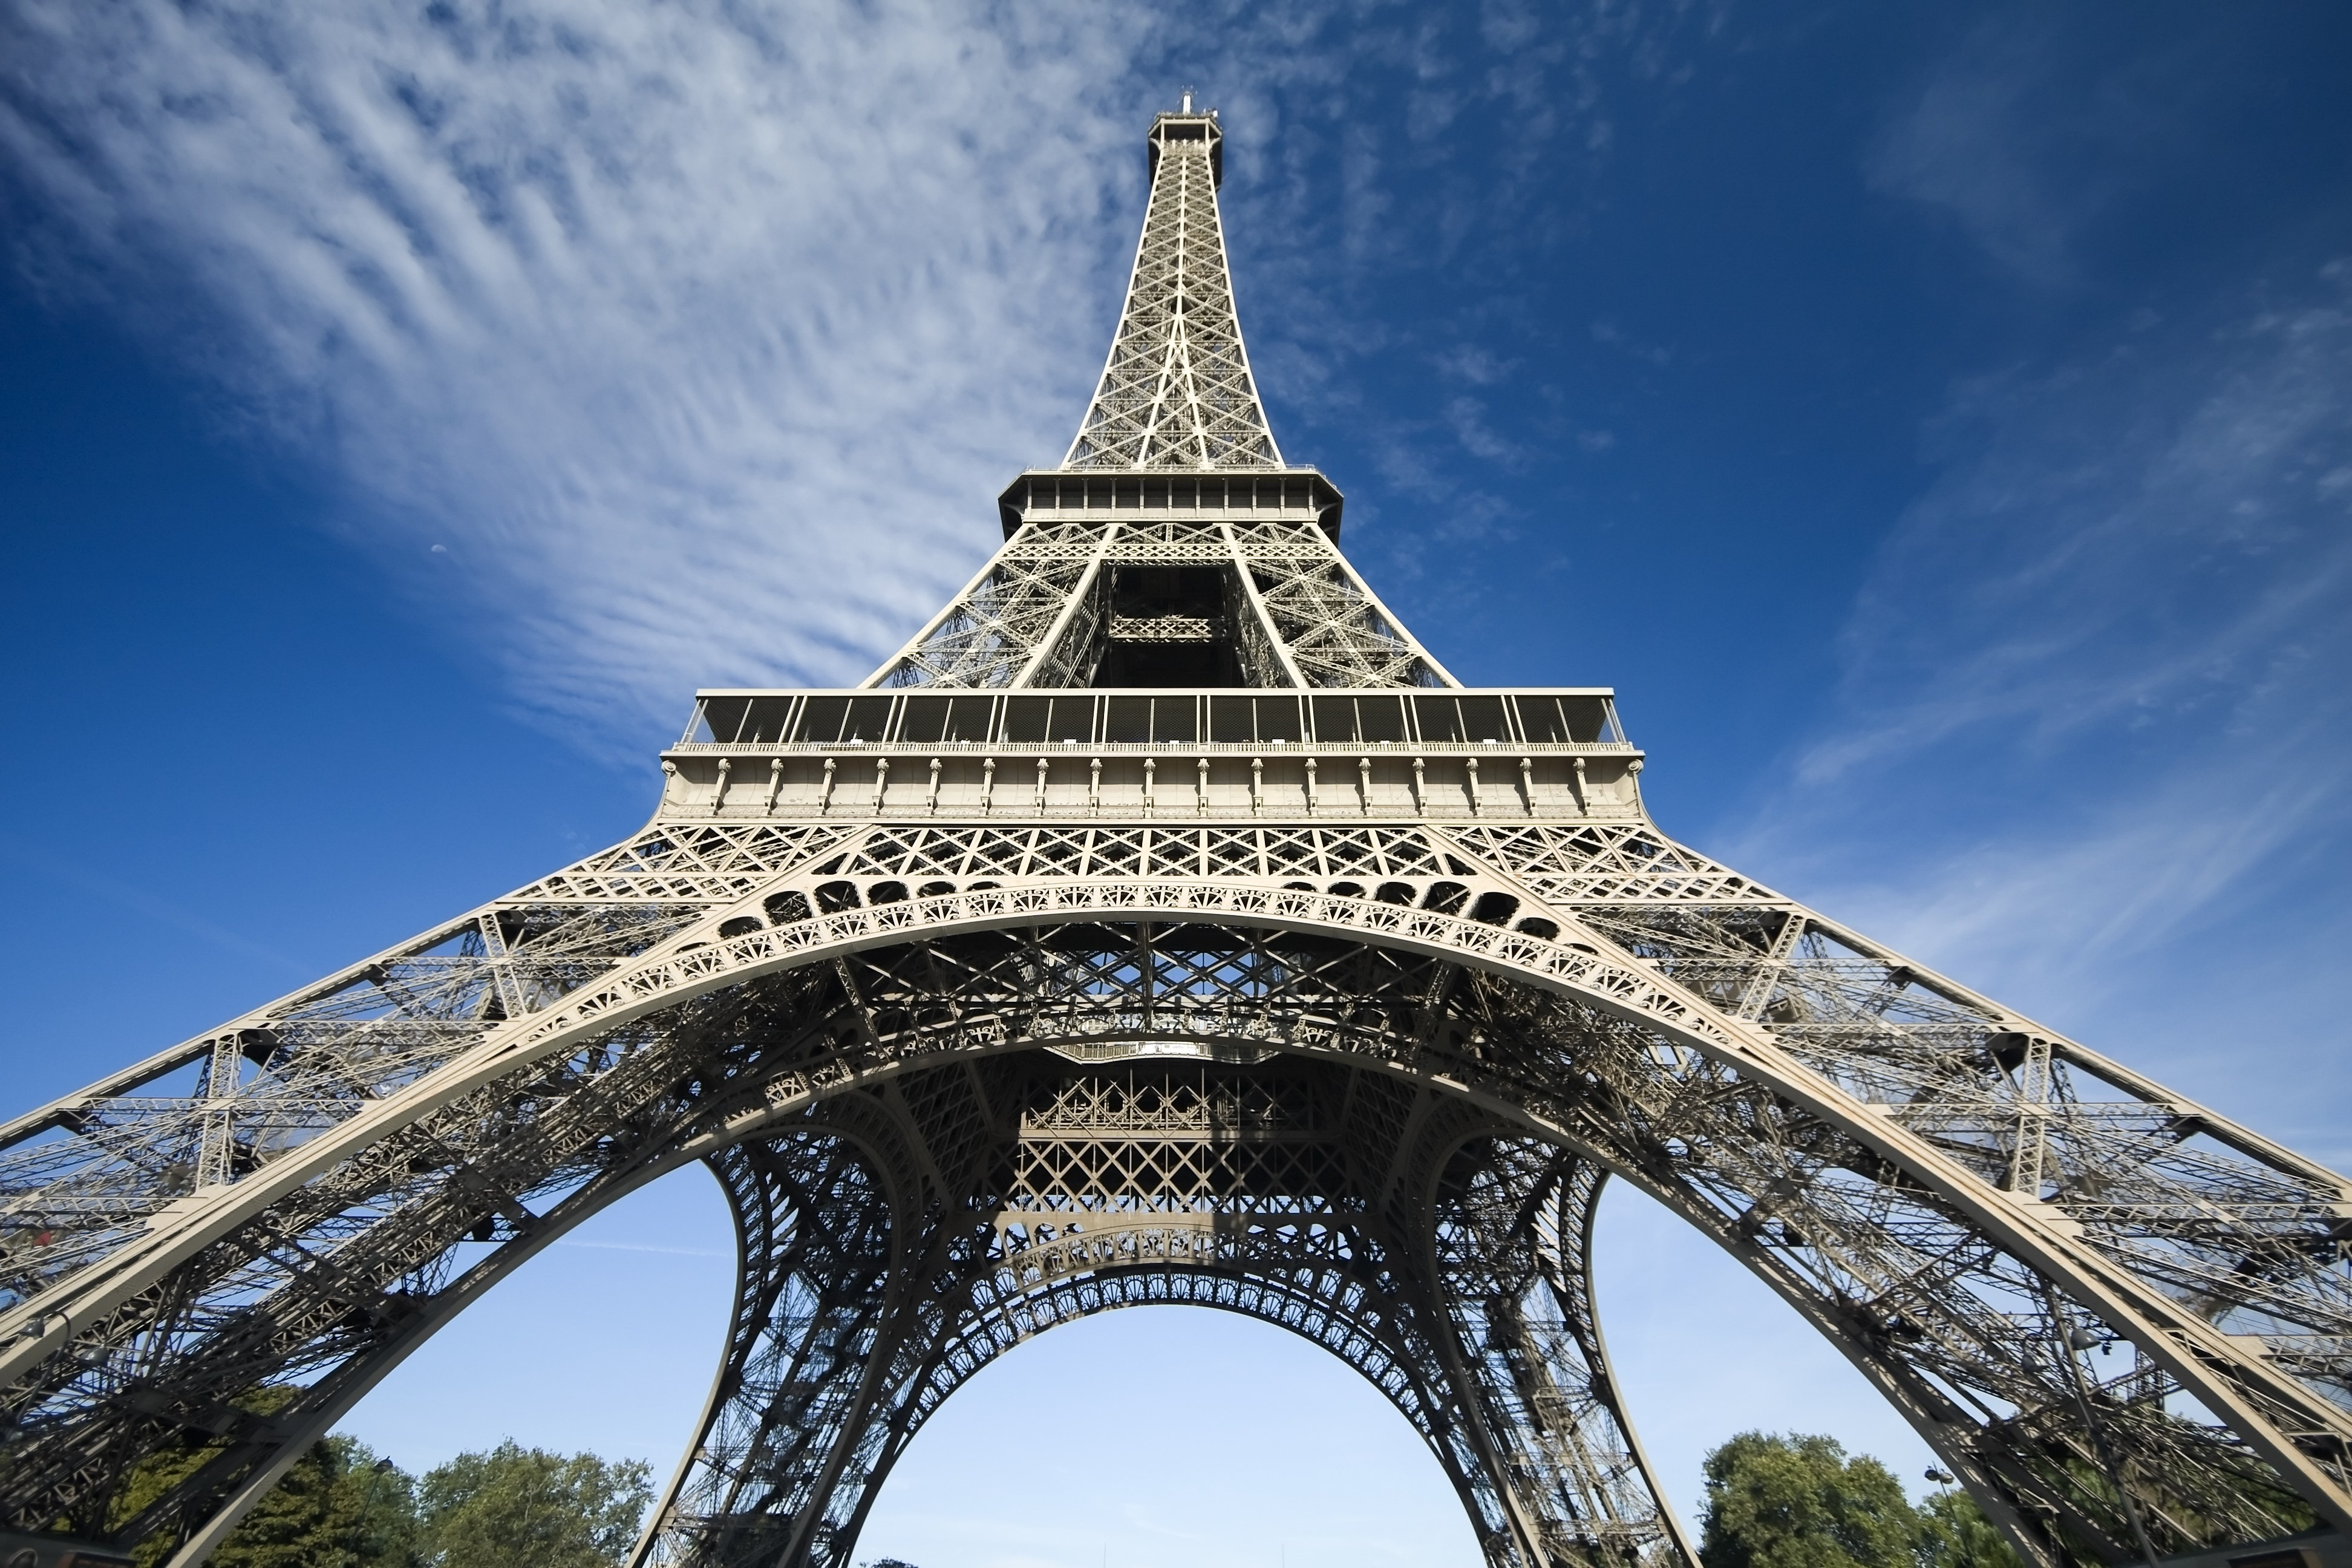
\includegraphics[width=\textwidth]{labwork8-gpu-out.jpg}
\bibliographystyle{plain}
\end{document}
